\documentclass[english]{beamer}
\usepackage[T1]{fontenc}
\usepackage[utf8x]{inputenc}
\setcounter{secnumdepth}{3}
\setcounter{tocdepth}{3}
\usepackage[authoryear]{natbib}
\usepackage{graphicx}
\usepackage{comment}

\makeatletter
%%%%%%%%%%%%%%%%%%%%%%%%%%%%%% Textclass specific LaTeX commands.
 % this default might be overridden by plain title style
 \newcommand\makebeamertitle{\frame{\maketitle}}%
 % (ERT) argument for the TOC
 \AtBeginDocument{%
   \let\origtableofcontents=\tableofcontents
   \def\tableofcontents{\@ifnextchar[{\origtableofcontents}{\gobbletableofcontents}}
   \def\gobbletableofcontents#1{\origtableofcontents}
 }

%%%%%%%%%%%%%%%%%%%%%%%%%%%%%% User specified LaTeX commands.
\title{DataSense: Data Intelligence}
%\subtitle{}

\usepackage{mymacros}

\makeatother

\usepackage{babel}
\begin{document}

\title[DataSense]{DataSense: Data Intelligence}
\author{C\'eline Hudelot \& Bertrand Thirion}
\institute[]{MICS Laboratory \& Inria Saclay} % Centrale-Supélec \& Inria
\date[DigiCosme Research Days]{DigiCosme Research Days\\ Gif, 5--6/6/2018}

\makebeamertitle

\begin{frame}{DataSense: Data Intelligence}
  \begin{columns}
    \begin{column}{7cm}
      
      \begin{itemize}
      \item Data are everywhere

        \begin{itemize}
        \item The Web, information systems, sensors (smartphones, etc.)
        \item Knowledge Graph, Wikipedia, WordNet...
        \end{itemize}
      \item Big data makes new things possible

        \begin{itemize}
        \item Statistical machine translation
        \item e-science
        \item Business intelligence
        \item ...
        \end{itemize}
      \end{itemize}
    \end{column}
    \begin{column}{3cm}
      
\includegraphics[width=\linewidth]{Images/digicosme.png}
    \end{column}
  \end{columns}
\end{frame}


%%% Local Variables: 
%%% mode: latex
%%% coding: utf-8-unix
%%% ispell-local-dictionary: "english"
%%% TeX-master: "datasense-2016.tex"
%%% fill-column: 9999
%%% End: 

\begin{comment}
%================================================================
\begin{frame}{Research Teams in DataSense}
%================================================================

  \begin{center}
    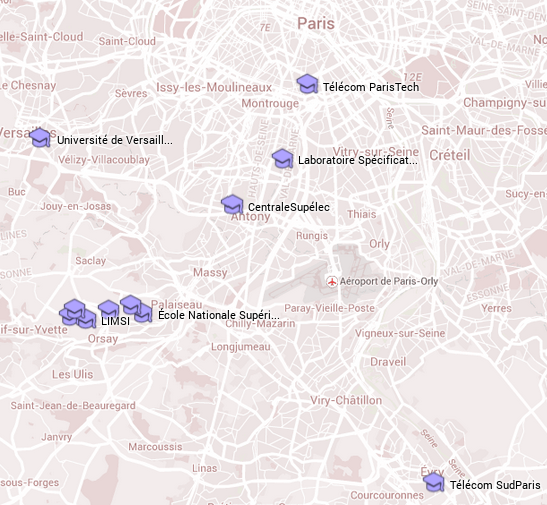
\includegraphics[width=.7\linewidth]{Images/datasense-locations.png}%
    \only<2>{\llap{\raisebox{1cm}{\fbox{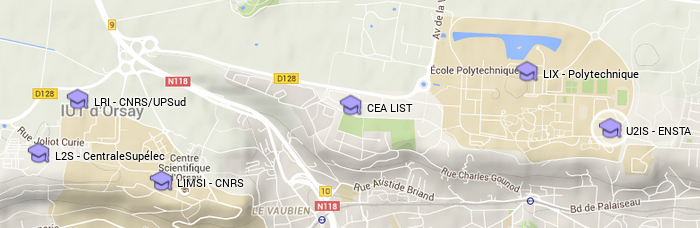
\includegraphics[width=.7\linewidth]{Images/datasense-orsay1.png}}\hspace*{1.5cm}}}}
  \end{center}

\end{frame}
\end{comment}

%================================================================
\begin{frame}{Research Teams in DataSense}

\begin{itemize}
\item \href{http://.david.uvsq.fr/}{DAVID} --- Université Versailles St Quentin
\item \href{http://www.inria.fr/centre/saclay }{Inria Saclay}
\item \href{http://www.l2s.centralesupelec.fr/}{L2S} --- Centrale-Supélec
\item \href{http://www.uvsq.fr/laboratoire-d-informatique-parallelisme-reseaux-algorithmes-distribues-li-parad}{Li-PaRAD} --- Université Versailles St Quentin
\item \href{https://www.limsi.fr/fr/}{LIMSI} --- CNRS – Université Paris-Sud
\item \href{http://www-list.cea.fr/}{LIST} --- CEA
\item \href{http://www.lix.polytechnique.fr/}{LIX} --- École Polytechnique
\item \href{http://lmv.math.cnrs.fr/}{LMV} --- Université Versailles St Quentin
\item \href{http://www.lsv.ens-cachan.fr/}{LSV} --- ENS – Cachan
\item \href{http://www.lri.fr/}{LRI} --- Université Paris-Sud
\item \href{https://www.ltci.telecom-paristech.fr/}{LTCI} --- Télécom Paris-Tech
\item \href{http://www.mics.ecp.fr/}{MICS} --- Ecole Centrale – Paris
\item \href{http://www.samovar.telecom-sudparis.eu/}{SAMOVAR} --- Télécom Paris-Sud
\item \href{http://u2is.ensta-paristech.fr/}{U2IS} --- Université Versailles St Quentin
\end{itemize}
\end{frame}

%%% Local Variables: 
%%% mode: latex
%%% coding: utf-8-unix
%%% ispell-local-dictionary: "english"
%%% TeX-master: "datasense-2016.tex"
%%% fill-column: 9999
%%% End: 


\begin{frame}{Plan}
\tableofcontents{}
\end{frame}

\section{Structuring}
\begin{frame}{DataSense `Tasks'}

\begin{enumerate}
\item Scalable, expressive and secure tools for large-scale data
\item Making sense of complex, heterogeneous data and knowledge
\item Machine learning: multi-task learning and meta-learning 
\item Distributed decision making: reinforcement learning, partially observable
processes and games
\item Interaction and Visualization
\end{enumerate}
\end{frame}

%%% Local Variables: 
%%% mode: latex
%%% coding: utf-8-unix
%%% ispell-local-dictionary: "english"
%%% TeX-master: "datasense-2016.tex"
%%% fill-column: 9999
%%% End: 


\section{Activities}
% Le découpage ci-dessous pourrait être revu : 
\begin{frame}{Global DataSense Activities}

  \begin{itemize}
  \item Main global activities:
    \begin{itemize}
    \item Research days (once a year)
    \item Community building
    \item Preparation of working groups and co-supervised theses
    \end{itemize}

  \item Activities per `Task'
    \begin{itemize}
    \item Working groups
    \item Co-supervised PhD theses
    \item Induced collaboration, Guest Scientists
    \end{itemize}

  \item Emerging projects: 
    \begin{itemize}
    \item SEDA: BREATHING SENSE INTO DATA
    \item Neural Meta Tracts
    \item IoTA Internet of Things Analytics
    \end{itemize}
  \end{itemize}

\end{frame}

%%% Local Variables: 
%%% mode: latex
%%% coding: utf-8-unix
%%% ispell-local-dictionary: "english"
%%% TeX-master: "datasense-2016.tex"
%%% fill-column: 9999
%%% End: 

\begin{frame}{DataSense Working Groups}
  \framesubtitle{Bottom-up creation of DigiCosme working groups}

%  \vspace*{-8mm}
%  \hspace*{-1cm}
%  \begin{columns}
%    \begin{column}[t]{6cm}
      \begin{itemize}
       \item {\small \textbf{ERVEN} : Extraction, Représentation et Visualisation de connaissance pour
l'Enseignement Numérique -- 2018 / 2019}
        \begin{itemize}
        \item Anne-Laure Ligizat
          % https://digicosme.lri.fr/tiki-index.php?page=GT+ERVEN
        \end{itemize}

        \item \textbf{E-santé} : Internet des Objets \& E-santé -- 2017 / 2019
        \begin{itemize}
        \item Mehdi Ammi
          % https://digicosme.lri.fr/tiki-index.php?page=GT+Internet+des+objets+et+E-sant%C3%A9
        \end{itemize}

        \item \textbf{TAL \& SEM} : TRAITEMENT SÉMANTIQUE DES DONNÉES TEXTUELLES -- 2017 / 2018
        \begin{itemize}
        \item  Brigitte Grau, LIMSI
          % https://digicosme.lri.fr/tiki-index.php?page=GT+TAL+et+SEM
        \end{itemize}

        \item \textbf{SDT} : Sécurité des Données Textuelles-- 2016 / 2017
        \begin{itemize}
        \item Cyril Grouin, LIMSI
          % https://digicosme.lri.fr/tiki-index.php?page=GT_SDT
        \end{itemize}

      \item D2K: From Data to Knowledge -- 2015/2017
        \begin{itemize}
        \item Claire Nédellec, INRA ; Chantal Reynaud, LRI 
        % \item http://labex-digicosme.fr/GT+D2K 
        \end{itemize}

        \item \textbf{SSSL} : Séquential Structured Statistical Learning – 2015 / 2017
          \begin{itemize}
          \item Oldaric Maillard, LRI
            % https://digicosme.lri.fr/tiki-index.php?page=GT+SSSL
          \end{itemize}
      \end{itemize}    
\end{frame}

\begin{frame}{DataSense Working Groups}
  \framesubtitle{Bottom-up creation of DigiCosme working groups}

%    \end{column}
%    \begin{column}[t]{6.5cm}
      \begin{itemize}    
      \item \textbf{SciCoSense:} Building a cartographic map of scientific communities -- 2015/2016
        \begin{itemize}
        \item Philippe Caillou, LRI
        % \item http://labex-digicosme.fr/GT+SciCoSense
        \end{itemize}

      \item \textbf{Human-Robot Interaction} -- 2015/2016
        \begin{itemize}
        \item Laurence Devillers \& Jean-Calude Martin (LIMSI-CNRS) 
        % \item http://labex-digicosme.fr/GT+Interaction 
        \end{itemize}

      \item \textbf{Deep Learning and Distributed Representations} -- 2014/2018
        \begin{itemize}
        \item Alexandre Allauzen, LIMSI 
        \item Emmanuelle Frenoux, LIMSI 
        % \item http://labex-digicosme.fr/GT+Reseaux+profonds 
        \end{itemize}

      \item \textbf{PASADENA}: Prédiction et Analyse de données structurées et hétérogènes -- 2015/2018
        \begin{itemize}
          \item Arthur Tenenhaus, Centrale-Supélec
          \item Maxime Sangnier, TPT 
          \item Flora Jay, LRI
        % \item http://labex-digicosme.fr/GT+PASADENA
        \end{itemize}

      \end{itemize}
%    \end{column}
%  \end{columns}
\end{frame}

\begin{frame}{Guest Scientists}

\begin{itemize}
\item 
\textbf{Kevin Bretonnel Cohen} - Director, Biomedical Text Mining Group Computational Bioscience
Program / University of Colorado School of Medicine  - Février / Avril 2016
\\
Contact : Pierre Zweigenbaum
%Séminaires : 3 GT (https://digicosme.lri.fr/tiki-index.php?page=GT+D2K+INTRANET,
%https://digicosme.lri.fr/tiki-index.php?page=GT+Representations+Semantiques+Multilingues,
%https://digicosme.lri.fr/tiki-index.php?page=GT+SciCoSense
% http://labex-digicosme.fr/Professeurs+Invites
\item 
\textbf{Catherine Plaisant} - University of Maryland Institute for Advanced Computer Studies -
Juin / Juillet 2017
\\
Contact : Jean-Daniel Feketé (Inria)
% Séminaires : http://visu2017.liris.cnrs.fr,
%http://www.aviz.fr/wiki/pmwiki.php/DayCourse2017/EventAnalytics,
%http://paris.sigchi.acm.org/homepage/home.php
\item
\textbf{Timothy Miller} - Boston Children's Hospital \& Harvard Medical School – Juin / Juillet 2017
\\
Contact : Aurélie Névéol (LIMSI)
\end{itemize}
\end{frame}

\begin{frame}{PhD students}

\begin{itemize}
\item 
\small
\textbf{HiDimStat} : Statistical control of sparse models in high dimension - 2017
\\
Bertrand Thirion (Inria) \& Joseph Salmon (LTCI)
% \\
% Doctorant /PhD Student : Jérôme Alexis CHEVALIER
\item
\textbf{Idiab} : Internet des Objets pour le suivi et la modélisation de la glycémie de patients
diabétiques - 2017
\\
Mehdi Ammi (LIMSI) \& XXX
%\\
% Doctorant / Phd student : Maxime De Bois
\item
\textbf{AlCoMol} : Algorithmique de graphes pour l’aide à la décision dans la construction
moléculaire – 2016
\\
Domnique Barth (DAVID)
% Doctorant / Phd student : Stefi Nouleho
\item 
\textbf{OPALE} : Opérateurs monotones aléatoires et applications à l’optimisation stochastique -
2015
\\
W. HACHEM, P. BIANCHI, J. JAKUBOWICZ, LTCI/ SAMOVAR
% Doctorant / Phd student : Adil SALIM
\item 
\textbf{COT} : Coréférence événementielle cross-document dans les dossiers électroniques
patient - 2015
\\
A. NÉVÉOL, X. TANNIER, O. FERRET, LIMSI / CEA-LIST
% Doctorant / Phd student :Julien TOURILLE
\item 
\textbf{SEDA} : BREATHING SENSE INTO DATA - 2015. Fabian Suchanek, LTCI
% Doctorant / Phd student : Thomas REBELE
\item 
\textbf{SensoMotor-CVE} : Murs d'images en contexte interactif complexe – 2015
\\
Patrick Bourdot, LIMSI
% Doctorante / Phd student : Yujiro OKUYA
\item
\textbf{BIPIMA} : BIPolarité de l'Information Multimédia pour l'Annotation sémantique d'images
dans un contexte de médias sociaux - 2014
\\
Céline Hudelot \& XXX  MICS / CEALIST / LTCI
% Doctorante / Phd student :Sonia A JINA
\end{itemize}
\end{frame}

\begin{frame}{Post-doc and engineers}

\small
\begin{itemize}
\item 
\textbf{MAEL} : MultimediA Entity Linking biologiques – 2018
\\
Contact : Hervé Le Borgne, CEA LIST
% Candidats : Omar Adiali
\item
\textbf{VASTE} :Veracity Assesment in Spatio-TEmporal heterogeneous data. 
% An application on Web animal epidemiological surveillance – 2018
\\
Contact : Fatiha Saïs, LRI
%Candidat : Joana Esther Gonzales Malaverri
\item
\textbf{MetaTracts} : Parsimonious multi-resolution representations for 
statistically analyzing brain tractograms – 2018
\\
Contact : Pietro Gori, LTCI – LIX
% Candidats : Pierre Roussillon
\item
\textbf{PASADENA} 
%: Prédiction et Analyse de données structurées hétérogènes 
– 2017
\\
Contact : Remy Boyer \& Franck Nielsen, L2S
% Candidats : Gia-Thuy PHAM - Romain Brault
\item
\textbf{AMPHI} : Approximate Message Passing for HIgh-dimensional data – 2017
\\
Contact : Bertrand Thirion, Inria \& Jospeh Salmon, LTCI
% Candidats : André Manoel
\item
\textbf{TAL \& SEM} : Traitement Sémantique des Données Textuelles - 2017
\\
Contact : Brigitte Grau \& Olivier Ferret, LIMSI
% Candidat : Marine Beltrix
\item
\textbf{D2K} : De la Donnée à la Connaissance - 2017
\\
Contact : Jean-Daniel Feketé, Inria
% Candidat : Christoph Kindeldey
\item
\textbf{SEDA} – 2015. Contact : Fabian Suchanek, LTCI
% Candidat : Camille Bourgaux
\end{itemize}
\end{frame}

\begin{frame}{Doctoral missions}

\begin{itemize}
\item
\textbf{
Plateforme Camomile d’annotation collaborative de documents multimédia} - 2016
Direction : Hervé BREDIN, LIMSI
% Doctorant : Romain Beaumont
% Institution : LIMSI
\url{https://github.com/camomile-project/camomile-polymer-client}
\item
\textbf{Software for easier access to open M/EEG data repositories} - 2016
Direction : Alexandre GRAMFORT; LTCI
% Doctorant : Mainak JAS
% Institution : LTCI
% Hébergement du code : 
\url{https://github.com/jasmainak/bids-validator}
\end{itemize}
\end{frame}

%%% Local Variables: 
%%% mode: latex
%%% coding: utf-8-unix
%%% ispell-local-dictionary: "english"
%%% TeX-master: "datasense-2016.tex"
%%% fill-column: 9999
%%% End: 


\begin{comment}
%================================================================
\begin{frame}{From Data to Knowledge}
\framesubtitle{Activities: 12 laboratories involved, 18 teams, 64 registered researchers, about 20 participants per meeting}

Meetings topics (including 2 national and 1 international speakers):
\begin{itemize}
\item Information extraction from texts, ontologies
\item Modeling and processes
\item Knowledge and image analysis
\item Knowledge and reasoning
\item Multimedia content analysis
\end{itemize}

\end{frame}
\end{comment}

%================================================================
\begin{frame}{From Data to Knowledge}
\framesubtitle{Contact: Claire Nedellec (INRA) \& Chantal Reynaud (LRI)}
\vspace{-5mm}
{\color{blue} \contacturl{http://labex-digicosme.fr/GT+D2K}}

Activities: 12 laboratories involved, 18 teams, 64 registered researchers, about 20 participants per meeting
%
\begin{itemize}
  \small
  \item[$\rightarrow$] \emph{CS for modeling living organisms} $\rightarrow$ priority topic in the Life Sciences Department SGT5
  \item[$\rightarrow$] Issued a document included in the \emph{Life Sciences Department White Paper}

\item Led to ANR-DFG project GoASQ (ANR-DFG: LRI-LIMSI-TUD, 2015--2019): \emph{Generating and Answering Ontological Queries over Semi-structured Data}
\item Contribution to the B2SRI Strategic Research Institute application
  \begin{itemize}
  \item Systems Biology and Synthetic Biology for Research and Innovation (Life Sciences + CS)
  \end{itemize}
\item Two teams collaborate in H2020 E-Infra OpenMinTeD: Open Mining Infrastructure for Text and Data (2015--2018)
\item DigiCosme Invited Professor: Kevin B.\ Cohen (U.\ Colorado), text mining in biomedicine (3 months, 2016)
\end{itemize}
\end{frame}


%================================================================
\begin{frame}{Building a cartographic map of scientific communities (SciCoSense) }
%================================================================
  \framesubtitle{Contact: Philippe Caillou, LRI}
\vspace*{-1cm}
{\color{blue}
\contacturl{http://labex-digicosme.fr/GT+SciCoSense}}
  \begin{columns}
    \begin{column}{4cm}
      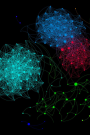
\includegraphics[width=\linewidth]{Images/scicosence-image.png}
    \end{column}
    \begin{column}{10cm}
      Representation and study of social networks:
      \begin{itemize}
      \item Study scientific communities
      \item based on traces of their activities
      \item to build indicators, maps and query tools
      \item about scientific production
      \end{itemize}
      \end{column}
  \end{columns}


\end{frame}

%================================================================
\begin{frame}{Deep Learning and Distributed Representations}
%================================================================
\framesubtitle{Contact: Alexandre Allauzen, LIMSI ; Emmanuelle Frenoux, LIMSI }
\vspace{-1cm}
{\color{blue} \contacturl{http://labex-digicosme.fr/GT+Reseaux+profonds}}
\begin{columns}
  \begin{column}{8cm}
    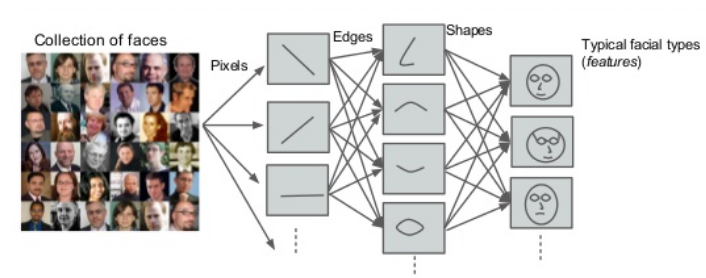
\includegraphics[width=\linewidth]{Images/dl.png}
  \end{column}
  \begin{column}{5cm}
    DataSense Task~3 (Machine learning)\\[2ex]
    
    \emph{Topic:}\\
    Deep neural networks and representation learning\\[2ex]
    
    \emph{Activities:}
    \begin{itemize}
    \item Journal club
    \item Cross-team presentations
    \item Invited seminars
    \end{itemize}
  \end{column}
  
\end{columns}
\vfill

  \emph{Participants:}\\
    LIMSI, CNRS (TLP, AMI) ---
    LRI, CNRS \& UPSud (TAO) ---
    U2IS, ENSTA ---
    LTCI, Télécom-ParisTech



\end{frame}


%================================================================
\begin{frame}{Prédiction et Analyse de données structurées et hétérogènes (PASADENA) }
%================================================================
\framesubtitle{Contact: 
Arthur Tenenhaus, Centrale-Supélec ; Maxime Sangnier, Télécom-ParisTech \&
Flora Jay, LRI}
\vspace{-5mm}
{\color{blue} \contacturl{ http://labex-digicosme.fr/GT+PASADENA}}

\begin{alertblock}{Objectives}
Developpement of statistical methods for complex data analysis: \textbf{heterogeneous}, \textbf{multimodal} and \textbf{structured} data:
\begin{itemize}
\item unsupervised analysis of correlations between modalities;
\item classification/regression from heterogeneous data;
\item structured prediction to fit a certain type of data from another;
\end{itemize}
\end{alertblock}


\begin{minipage}[c]{.7\linewidth}
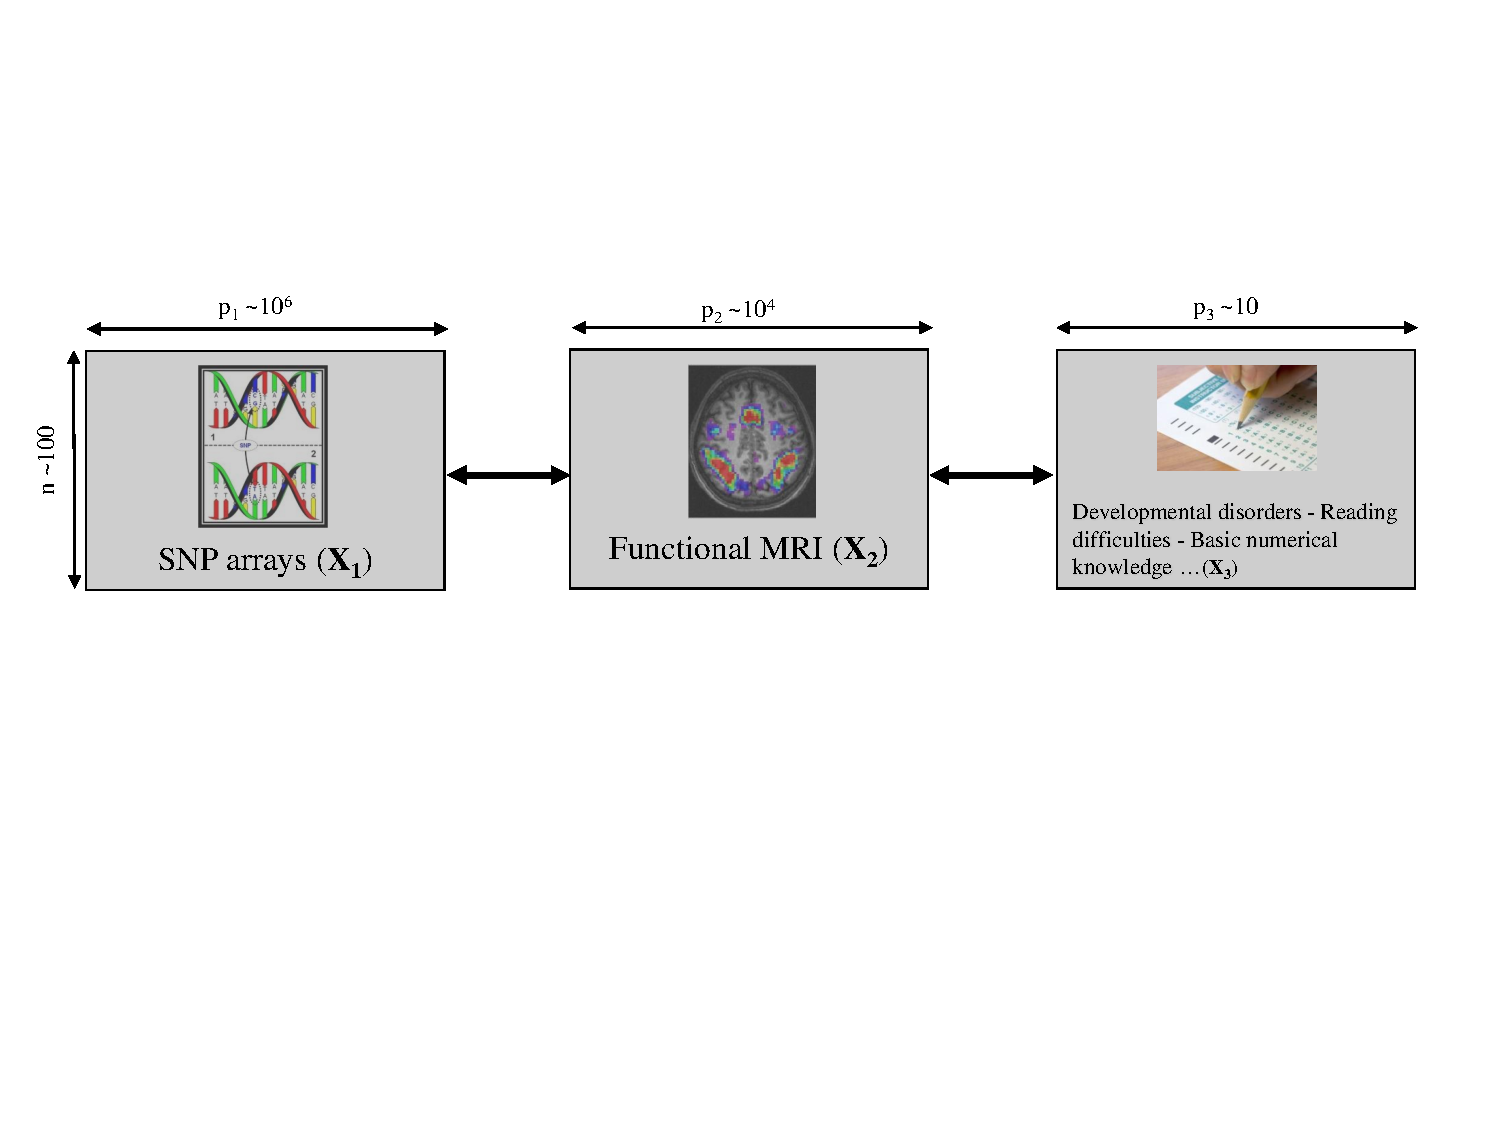
\includegraphics[trim = 0mm 90mm 0mm 50mm, clip, width=\linewidth]{Images/pasadena_poster_I.pdf}
\end{minipage}\hfill
\begin{minipage}[c]{.28\linewidth}
Multibloc study in imaging genetics.
\end{minipage}


\end{frame}



%================================================================
\begin{frame}{Human-Robot Interaction}
%================================================================
\framesubtitle{Contact: Laurence Devillers \& Jean-Calude Martin (LIMSI-CNRS) }
{\color{blue} \contacturl{http://labex-digicosme.fr/GT+Interaction}}

\begin{minipage}[c]{.35\linewidth}
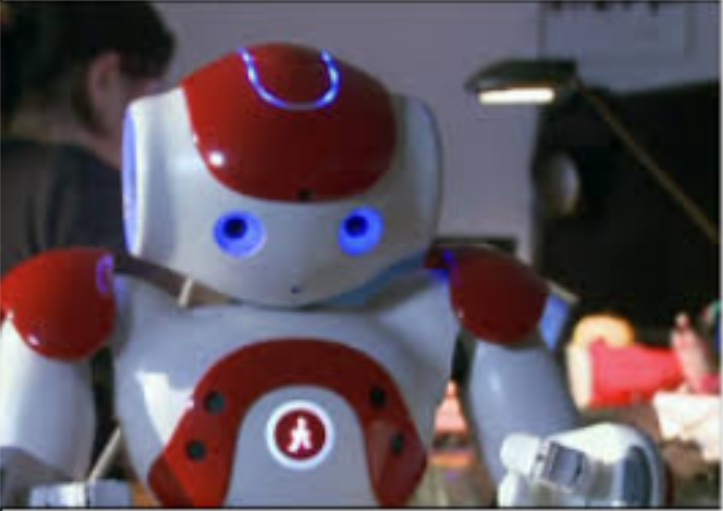
\includegraphics[width=\linewidth]{Images/hr1.png}
\end{minipage} 
\hfill
\begin{minipage}[c]{.64\linewidth}
Objectives
\begin{itemize} 
\item Create a community on interactive robotics; verbal/non-verbal/physical Human-robot interactions 
\item Group specialists beyond robotics: modeling and interaction, big data, psychology, social and cognitive sciences, ergonomy and  usage, ethics.
\end{itemize}
 Members : LIMSI, ENSTA, CEA, Télécom SudParis, Télécom ParisTech, Télécom Ecole de Management, Université Paris-Sud, UVSQ, Université d’Evry, CERDI
\end{minipage}


\end{frame}


%================================================================
\begin{frame}{ERVEN : Extraction, Représentation et Visualisation de connaissance pour
l'Enseignement Numérique}
\framesubtitle{Contact: Anne-Laure Ligizat}
{\color{blue} \contacturl{https://digicosme.lri.fr/tiki-index.php?page=GT+ERVEN}}
\begin{columns}
  \begin{column}{7cm}
    \hspace*{-1cm}
    \begin{itemize}
    \item Équipes du LIMSI :
      \begin{itemize}
      \item
        Équipe ILES (Brigitte Grau, Gabriel Illouz, Anne-Laure Ligozat)
      \item
        Équipe AMI (Frédéric Vernier)
      \item
        Équipe TLP (Alexandre Allauzen) 
      \end{itemize}
    \item Équipes du LRI : 
      \begin{itemize}
      \item LaHDAK: Philippe Dague,
        Yue Ma, Brigitte Safar, Fatiha Saïs 
      \item MODHEL:Yolaine Bourda, Fabrice Popineau
      \end{itemize}
    \item SAMOVAR, Telecom SudParis :
      Amel Bouzeghoub 
    \end{itemize}
  \end{column}
  \begin{column}{6cm}
    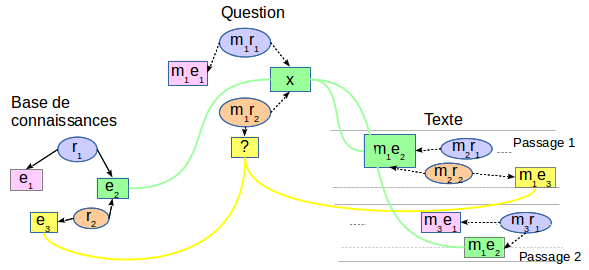
\includegraphics[width=6cm]{Images/education.png}
  \end{column}
\end{columns}
\end{frame}


\begin{frame}{E-santé : Internet des Objets and E-santé -- 2017 / 2019}
\framesubtitle{Contact : Mehdi Ammi}
%
\vspace{-1cm}
\hspace*{-5mm}
{\color{blue} \contacturl{https://digicosme.lri.fr/tiki-index.php?page=GT+Internet+des+objets+et+E-sante}}
%
%
\begin{columns}
  \begin{column}{5.5cm}
    \begin{itemize}
    \item étude, conception et évaluation des services e-sant\'e
    \item traitement des données
    \item technologie
    \item éthique
    \end{itemize}
  \end{column}
  %
  \begin{column}{7cm}
    \begin{itemize}
    \item Laboratoires \textit{TIC}: LIMSI( AMI, CPU, ILES, TLP),
      ENSTA ParisTech, CIAMS, Telecom SudParis, CEA-LIST, LRI
    \item Laboratoire \textit{Santé} End-icap Fondation Helene -
      Poidatz Handiresp Hôpital Bicêtre
    \item \textit{Associations et pôles}: RevesDiab France eHealthTech
      Systematic Capdigital OpticsValley Fedev (SFR)
    \end{itemize}
  \end{column}
\end{columns}
\end{frame}


\begin{frame}{ TAL \& SEM : Traitement sémantique des données textuelles – 2017 / 2018}
\framesubtitle{Contact : Brigitte Grau, LIMSI}
\vspace{-1cm}
{\color{blue} \contacturl{https://digicosme.lri.fr/tiki-index.php?page=GT+TAL+et+SEM}}
\\
Implication textuelle, paraphrase, désambiguisation sémantique

\begin{columns}
\begin{column}{8cm}
\begin{itemize}
\item \textbf{Timothy Miller}: Boston Children's Hospital, Introduction to sequence models for Natural Language Processing
\item \textbf{Brigitte Grau}: LIMSI, De la recherche de réponses à des questions à la compréhension ciblée de textes
\item \textbf{Olivier Ferret}: Apprentissage de connaissances sémantiques : adaptation de plongements lexicaux (words embeddings) à des connaissances externes
\end{itemize}
\end{column}
\begin{column}{5cm}
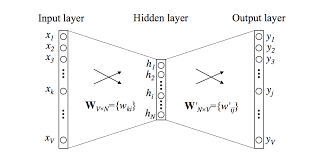
\includegraphics[width=5cm]{Images/language.png}
\end{column}
\end{columns}
\end{frame}

\vspace{-1cm}
\begin{frame}{SDT : Sécurité des Données Textuelles – 2016 / 2017}
\framesubtitle{Contact : Cyril Grouin, LIMSI}
{\color{blue} \contacturl{https://digicosme.lri.fr/tiki-index.php?page=GT_SDT}}

Common group with Scilex
\begin{columns}
\begin{column}{8cm}
\begin{itemize}
\item LIMSI : équipe ILES (Cyril Grouin (CNRS), Thomas Lavergne (Université Paris-Sud), Aurélie Névéol (CNRS), Pierre Zweigenbaum (CNRS)
\item INRIA-LIX : équipe COMETE (Catuscia Palamidessi, Kostantinos Chatzikokolakis)
\item CEA-LIST, équipe LVIC (Olivier Ferret, Gaël de Chalendar)
\end{itemize}
\end{column}
\begin{column}{5cm}
\begin{itemize}
\item
Anonymisation et risques de réidentification
\item
Protection des données dans les modèles
\item
Optimisation de la confidentialité différentielle
\end{itemize}
\end{column}
\end{columns}
\end{frame}

\begin{frame}{SSSL : Séquential Structured Statistical Learning – 2015 / 2017}
\framesubtitle{Contact : Oldaric Maillard, LRI}
{\color{blue} \contacturl{ https://sites.google.com/site/groupedetravailsssl/home}}
\begin{columns}
\begin{column}{10cm}
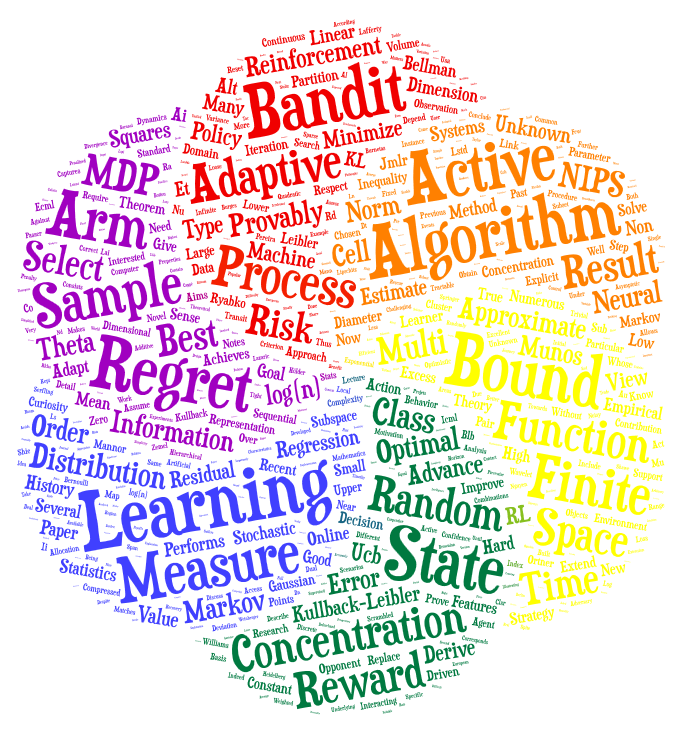
\includegraphics[width=6cm]{Images/Cloud-13.png}
\end{column}
\end{columns}
\end{frame}



\section{Perspectives}
\begin{frame}{Plan}
\tableofcontents{}[currentsection]
\end{frame}

%================================================================
\begin{frame}{DataSense Perspectives}

{Continue to build a community}
\begin{itemize}
\item In each activity:
\begin{itemize}
\item Emerging projects
\item Idex chairs
\item Bottom-up Working Groups\\
  are the driving force of collaborative work
\end{itemize}

\item 
Connect researchers beyond their specific domain

\begin{itemize}
\item Foster cross-domain inspiration and reuse of methods
\item Beyond tasks
\item Beyond action lines
\end{itemize}
\end{itemize}
\end{frame}


%================================================================
\begin{frame}{DataSense Perspectives}

Co-organized Seminars,
expressed as problems which require two types of expertise, e.g.:

\begin{itemize}
% \item I have collected 72 million forum messages with various metadata and links: how do I best store and query these data?
% \item I was given a heap of unstructured Web pages from which I must collect person names: how do I do?
\item Machine Learning+Heterogeneous data and knowledge:
  What kind of neural network should I train to merge word and concept spaces?
  % to index texts with ontological concepts?
% \item I want to record user interactions with my system: what are the best practices?
\item Knowledge+Visualization: What kinds of visualizations can help me explore an ontology with six million concepts?
% \item Which graph algorithms best find similar nodes in graphs of words?
\item Security+Text: How can I assess the risk of re-identification of a de-identified text corpus?

\item  Towards co-construction of joint projects
\end{itemize}

Shared Tasks

\begin{itemize}
\item In collaboration with the Center for Data Science, DataIA.
\item Objective: Define together cross-domain datasets and shared tasks
\end{itemize}
\end{frame}

%================================================================
\begin{frame}[plain]{}

  \vfill
  \begin{center}
    \huge THANK YOU!
  \end{center}
  \vfill

\end{frame}

%%% Local Variables: 
%%% mode: latex
%%% coding: utf-8-unix
%%% ispell-local-dictionary: "english"
%%% TeX-master: "datasense-2016.tex"
%%% fill-column: 9999
%%% End: 


\end{document}


%%% Local Variables: 
%%% mode: latex
%%% coding: utf-8-unix
%%% ispell-local-dictionary: "english"
%%% TeX-master: t
%%% fill-column: 9999
%%% End: 
